\begin{center}

  \begin{tabular}{rp{6cm}lp{12cm}}%{rl}

  % after \\: \hline or \cline{col1-col2} \cline{col3-col4} ...

  论文地址:& \href{https://arxiv.org/abs/1806.02473}{https://arxiv.org/abs/1806.02473} \\

\textbf{}  源码:& \href{https://github.com/bowenliu16/rl_graph_generation}{rl\_graph\_generation} \\

%  slides:& \href{http://yunshengb.com/wp-content/uploads/2017/03/nips_2018_r2l_workshop_talk.pdf}{{\footnotesize Convolutional Set Matching for Graph Similarity}}\\

  关键词:& \textbf{Graph Generation, Molecular Graph, Reinforcement Learning} \\

  写于:& \date{2020-10-21}

  \end{tabular}

\end{center}

该论文\cite{you2019graph}主要针对的是指定目标下的图生成问,论文的主要面向领域是药物发现,目的是生成满足某种属性以及约束条件的图。针对这个问题,论文提出了GCPN(Graph Convolutional Policy Network) --- 一种强化学习模型,通过策略梯度(policy gradient)来优化指定领域的奖励和对抗损失,在领域特定的约束环境中生成符合要求的图。

\begin{figure}[h]
	\centering
	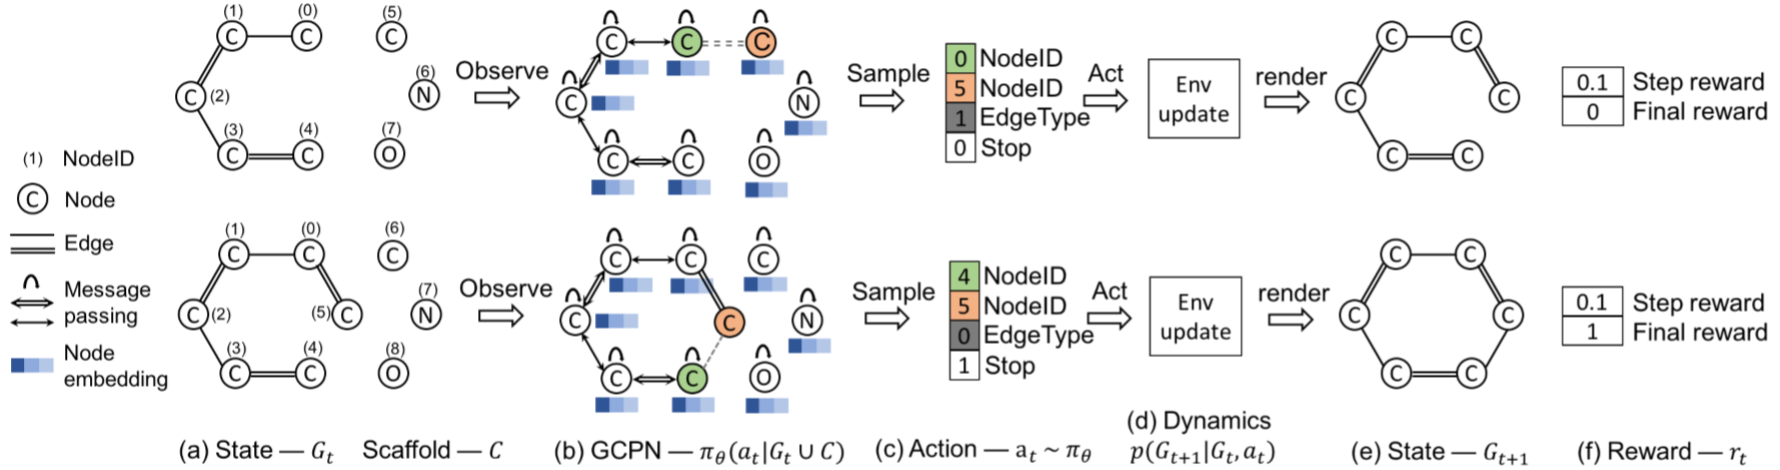
\includegraphics[width=.83\textwidth]{pics/GCPN.PNG}
	\caption{Overview of GCPN}
	\label{fig:gcpn}
\end{figure}

\paragraph{GCPN思路}整体过程如Fig.\ref{fig:gcpn}所示。在生成一个分子的过程中,是逐步通过将子结构连接到分子中或者添加边来完成的。生成一个有效分子的过程可以视作马尔可夫决策过程,从最起始的分子开始,通过执行动作进行状态转移,每个分子就是一个状态。其中,最重要的就是如何选取动作,即在每个状态下执行什么样的动作:$p(a_t | s_0,...,s_t)$,那么下一个状态就是:$p(s_{t+1} | s_0,...,s_t, a_t)$。论文中通过策略网络(policy network)来模拟$p(a_t | s_0,...,s_t)$。生成一个动作$a_t$后,会经过一些药物/化学方面的检验,来决定是否执行$a_t$,如果执行则会增加reward(即强化学习中的reward)。

需要强调的是,GCPN是通过RL来训练的,训练时不仅要考虑生成的动作是否符合要求还要考虑最后生成的分子是否满足某些性质及满足的程度。


\paragraph{方法解决的问题/优势}
\begin{itemize}
	\item 以目标导向的图生成问题来解决药物合成的问题,并且能满足药物需要满足的性质
	\item 以RL agent来对药物空间进行探索,生成的药物不一定与训练数据的分布一致,因为新的分子可能与训练数据的分布有较大差别,但是满足分子应有性质
	\item \tbc{red}{将不可微的分子的属性和一些先验条件加入到模型中}监督模型的训练,使模型向期望的方向发展

\end{itemize}



\paragraph{方法的局限性/未来方向}
\begin{itemize}
	\item 可以将模型应用到更广的范围,按照先验条件生成符合指定条件的图数据
	%\item 

\end{itemize}




